\section{An audit of published critical values in size units}\label{sec:audit}

A published critical value $\hat c$ for nominal level $\alpha$ is judged by the size it actually delivers,
$P(\text{statistic}>\hat c)$ under the law it is meant for, not by its relative error: near the tail of a heavy-tailed
law a $1\,\%$ error in $\hat c$ can be negligible or important depending on the density there. For every value in the
ledger (\cref{app:audit}) we record the source, page and table; the statistic and its normalisation (\cref{tab:norm});
the tail; the simulation design and number of replications $N$; and the version of the document that was read. We
then compute the true size, certified where the law is certified, and compare its deviation from $\alpha$ with the Monte
Carlo standard error of the source's own design, $\sqrt{\alpha(1-\alpha)/N}$. The verdict rules were fixed before the
computation: a value is \emph{accurate within Monte Carlo error} if its size deviation is within three standard errors.
The protocol allowed the word \emph{inaccurate} for deviations that the stated design does not explain or that exceed
$0.1$\,pp at the $5\,\%$ level; we use it only in the first, stricter sense, for values more than three standard errors
from nominal under the law they are meant for (class~E), and describe the others by their class. Each value receives
one of five classes, assigned in this order. A value more than three standard errors from nominal in the limit is in
class~(C) if it is within three standard errors under the exact law of a finite design that we infer the source
simulated, and in class~(E) otherwise. A value within three standard errors is in class~(D) if its block (one source,
statistic and memory regime, $H=\frac12$, $H>\frac12$ or $H<\frac12$) has at least three values, all within three standard
errors, all deviating in one direction, with standardised sum $|\sum_iz_i|/\sqrt k>3$, where $z_i$ is a deviation in
standard errors; otherwise it is in class~(B) if at the $5\,\%$ level it misses $5\,\%$ by more than $0.1$\,pp, and in
class~(A) if not. Classes~C and~D were added after the patterns described below had been seen, and are reported as
such. The standardised sum treats the values of a block as independent, but the values in one row of a table are
usually quantiles of one simulated sample; class~D therefore marks a one-sign pattern, not a deviation established
beyond Monte Carlo error.

\begin{figure}[tbp]\centering
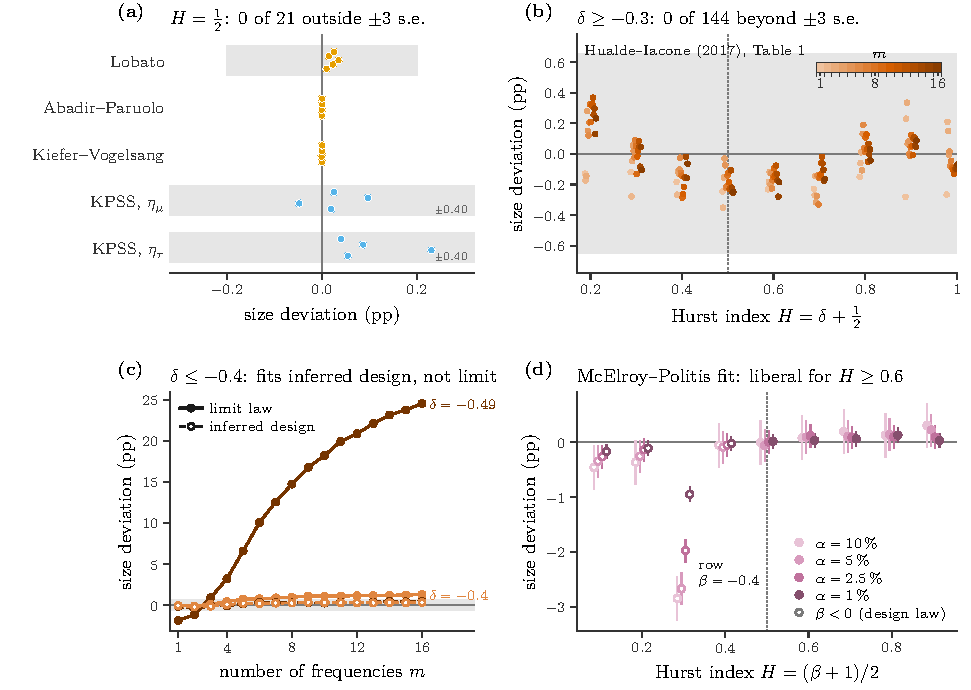
\includegraphics[width=\textwidth]{fig4_audit.pdf}
\caption{Size deviation of published critical values (pp); grey: $\pm3$ Monte Carlo standard errors of each
source's design. (a)~Sources at $H=\frac12$. (b)~\citet[Table~1]{HI17}, $\delta\ge-0.3$. (c)~Same table,
$\delta=-0.49$, $-0.4$: limit (filled), inferred finite design (open). (d)~\citet{MP09}: limit (filled), their
design (open); bars: $\pm3$ raw-quantile standard errors (reference scale, not a bound).}\label{fig:audit}
\end{figure}

\paragraph{$H=\frac12$} The values of \citet{AP97} and \citet{KV02} are exact to the printed digits: the largest
relative difference from the closed-form quantiles is \pthree{audit-apkv-maxrel}. The row $K=1$ of \citet[Table~1]{Lob01}
delivers sizes \pthree{audit-lob-sizes}\,\% at nominal $10$, $5$, $2.5$, $1$ and $0.5\,\%$, all within the Monte Carlo
error of the published design. For the stationarity statistics of \citet{KPSS92}, a bridge functional at $H=\frac12$,
the values for $\eta_\mu$ are accurate within Monte Carlo error, while the $5\,\%$ value $0.146$ for $\eta_\tau$ has size
\pthree{audit-kpss-tau-05}\,\%, \pthree{audit-kpss-tau-05-z} standard errors above nominal; the exact $5\,\%$ point is
\pthree{audit-kpss-tau-05-exact}.

\paragraph{Fixed-$m$ values of \citet{HI17}} Their Table~1 gives $176$ two-sided $5\,\%$ values for
$\delta=H-\frac12\in[-0.49,0.49]$ and $m=1,\dots,16$, from $10\,000$ replications in which the integrals of the limit
are replaced by sums over $10\,000$ steps (their Remark~6). For $\delta\ge0$ the true sizes range from
\pthree{audit-hi-pos-min} to \pthree{audit-hi-pos-max}\,\%; none of the \pthree{audit-hi-pos-n} values is more than two
standard errors from $5\,\%$, but \pthree{audit-hi-pos-gt01} of them miss $5\,\%$ by more than $0.1$\,pp. At $\delta=0$,
where the limit law is Student's $t$ with $2m$ degrees of freedom, all \pthree{audit-D-hi0-n} values are conservative,
with sizes from \pthree{audit-D-hi0-min} to \pthree{audit-D-hi0-max}\,\% (largest $|z|$ \pthree{audit-D-hi0-maxz}); their
standardised sum is \pthree{audit-D-hi0-jointz} (class~D), but the sixteen values share the replications of one
simulation, and treated as a single observation the row deviates by \pthree{audit-D-hi0-rowz} standard errors. For $\delta<0$,
certified through \cref{prop:continuation}, the limit sizes range from \pthree{audit-hi-neg-min} to
\pthree{audit-hi-neg-max}\,\%, and \pthree{audit-hi-neg-gt3se} of the \pthree{audit-hi-neg-n} values are more than three
standard errors from $5\,\%$ (\pthree{audit-hi-neg-gt2se} more than two). All of these are at $\delta=-0.49$ and $-0.4$, where the deviation grows with $m$: at
$\delta=-0.49$ the published value for $m=1$ has limit size \pthree{audit-hi-neg-m1-limit}\,\% and the one for $m=16$
has \pthree{audit-hi-neg-m16-limit}\,\%. The published values are nevertheless consistent with a finite design that could
have produced them. Under the exact law of the statistic computed from a stationary ARFIMA$(0,\delta,0)$ path of $10\,000$
observations, their sizes range from \pthree{audit-hi-neg-design-min} to \pthree{audit-hi-neg-design-max}\,\%, only
\pthree{audit-hi-neg-design-gt2} of the $80$ values are more than two standard errors from $5\,\%$, and none is more than
three (largest $|z|$ \pthree{audit-hi-neg-design-maxz}); a fractional Gaussian noise path of the same length gives
\pthree{audit-hi-neg-m16-fgn}\,\% at $\delta=-0.49$, $m=16$, close to the limit. Near $\delta=-\frac12$ the discretised
law approaches its limit extremely slowly: at $\delta=-0.49$ and $m=16$ the published value has size
\pthree{audit-hi-neg-m16-T1e3}, \pthree{audit-hi-neg-m16-T1e4} and \pthree{audit-hi-neg-m16-T1e5}\,\% for ARFIMA paths
of $10^3$, $10^4$ and $10^5$ observations. Their Remark~6 gives the number of steps but not the process that generated
the increments; the ARFIMA design is our inference from this match, so class~C is a statement about an inferred design.
The values are accurate for that design but are not limit critical values, and for strongly antipersistent series the critical value
must be taken from the exact finite-sample law at the actual $n$ (\cref{prop:exactn}). For $\delta\ge-0.3$ the table is
accurate to its Monte Carlo precision of about $\pm$\pthree{audit-hi-2se}\,pp in size, which is larger than the effect
of $\delta$ on the critical value at small $|\delta|$; the certified values replace it (\cref{app:tables}).

\paragraph{Bartlett values of \citet{MP09}} McElroy and Politis do not print simulated quantiles: for each kernel and
memory parameter $\beta=2H-1$ they print the coefficients of a polynomial fit of the $\log$ critical value in the
bandwidth ratio $b$. The Bartlett values at $b=1$ that we audit are therefore \emph{fitted values}, reconstructed from
the printed coefficients as $\exp(\sum_ia_i)$, and the error of the fit is part of what is measured. As the reference
scale we use the standard error of a raw simulated quantile at their $N=50\,000$; the uncertainty of a fitted value can
be smaller, because the fit pools neighbouring values of $b$, or larger, because the fit may be biased at the end point
$b=1$. At $H=\frac12$ the fitted
values deliver sizes within Monte Carlo error. For $H\ge0.6$ all \pthree{audit-mp-pos-n} values are too small: each is
within three standard errors (largest $z$ \pthree{audit-mp-pos-maxz}), but all \pthree{audit-mp-pos-npos} excesses are
positive, between \pthree{audit-mp-pos-min} and \pthree{audit-mp-pos-max}\,pp, and at $H=0.9$ and nominal $10\,\%$ the
size is \pthree{audit-mp-H090-a10}\,\% (class~D, standardised sum \pthree{audit-D-jointz}). The four levels of a row are
quantiles of one simulated sample; counting each of the \pthree{audit-D-nrows} rows as one observation, the excess is
\pthree{audit-D-jointz-rows} standard errors, so the pattern is suggestive rather than established. The excess does not
come from discretisation, because the exact law of
their $1000$-step design gives the same sizes; it may come from the polynomial smoothing at the end point $b=1$, which
we cannot verify from the report. For $\beta<0$ we compare with the exact finite-sample law of their discretised
design. The row $\beta=-0.4$ ($H=0.3$) is inaccurate: its size deviations reach \pthree{audit-mp-T3-dev10}\,pp at
nominal $10\,\%$, the size at nominal $5\,\%$ is \pthree{audit-mp-T3-size05}\,\%, and the deviations are up to
\pthree{audit-mp-T3-maxz} standard errors; the row is also non-monotone in $\beta$ at the upper levels, which is consistent with, but not proof of, a
transcription error in one printed coefficient; the report does not allow us to check this. Rounding of the printed
coefficients to three decimals does not explain it: it moves the size by at most \pthree{audit-mp-T3-round-maxshift}\,pp,
against deviations of \pthree{audit-mp-T3-round-mindev}\,pp and more. The row $\beta=-0.8$ deviates by \pthree{audit-mp-T1-devmin} to
\pthree{audit-mp-T1-devmax}\,pp, \pthree{audit-mp-T1-minz}--\pthree{audit-mp-T1-maxz} standard errors (class~E,
conservative); the rows $\beta=-0.6$ and $-0.2$ are within Monte Carlo error.

\paragraph{Summary} Of the \pthree{audit-n-values} audited values (the \pthree{audit-n-dup} values of the 1990 KPSS working
paper, identical to those of the article, are counted once), \pthree{audit-n-AB} are within three standard errors
of nominal in the law they are meant for (classes A and B), \pthree{audit-n-C} are consistent with a finite design that
we infer their source simulated but not with the limit (C), \pthree{audit-n-D} share a one-sign pattern within Monte
Carlo error (D), and
\pthree{audit-n-E} are more than three standard errors from nominal (E), all of them fitted McElroy--Politis values
at $\beta<0$; \cref{tab:audit} lists the classes by source and \cref{app:audit} every value. Two messages follow for the
user of a table. Monte Carlo precision of $\pm0.2$ to $\pm0.4$\,pp in size is all that most published tables deliver,
and \pthree{audit-n-B} values miss $5\,\%$ by more than $0.1$\,pp for that reason alone. And for the long-memory tables
the systematic component, whether from the fit or from the simulated design, can be larger than the Monte Carlo error.

\begin{table}[tbp]\centering\small
\caption{Verdicts by source. Deviation: true size minus nominal (pp); s.e.: Monte Carlo standard error of the
source's design; classes as in the text. \textsuperscript{a}No Monte Carlo error. The 1990 KPSS working paper,
identical to the article, is counted once.}\label{tab:audit}
\begin{tabular}{@{}llrrrrrrrr@{}}\toprule
& & & & & \multicolumn{5}{c}{verdict class}\\\cmidrule(l){6-10}
source & range & $N$ & deviation (pp) & s.e.\ (pp) & A & B & C & D & E\\\midrule
Lobato~\fixcite{Lob01} & $H=\frac12$ & 5 & +0.01 to +0.03 & 0.02--0.07 & 5 & -- & -- & -- & --\\
Abadir--Paruolo~\fixcite{AP97} & $H=\frac12$ & 4 & -0.00 to +0.00 & exact\textsuperscript{a} & 4 & -- & -- & -- & --\\
Kiefer--Vogelsang~\fixcite{KV02} & $H=\frac12$ & 4 & -0.00 to +0.00 & exact\textsuperscript{a} & 4 & -- & -- & -- & --\\
KPSS~\fixcite{KPSS92} & $H=\frac12$ & 8 & -0.05 to +0.23 & 0.04--0.13 & 7 & 1 & -- & -- & --\\
Hualde--Iacone~\fixcite{HI17} & $\delta\ge0$ & 96 & -0.35 to +0.34 & 0.22 & 36 & 44 & -- & 16 & --\\
Hualde--Iacone~\fixcite{HI17} & $\delta<0$ & 80 & -1.87 to +24.53 & 0.22 & 16 & 36 & 28 & -- & --\\
McElroy--Politis~\fixcite{MP09} & $\beta\ge0$ & 20 & -0.06 to +0.31 & 0.04--0.13 & 4 & -- & -- & 16 & --\\
McElroy--Politis~\fixcite{MP09} & $\beta<0$ & 16 & -2.85 to -0.02 & 0.04--0.13 & 7 & 1 & -- & -- & 8\\
\midrule all & & 233 & & & 83 & 82 & 28 & 32 & 8\\
\bottomrule\end{tabular}
%
\end{table}
